\StartPlate{V21}{A square table does not specify an entire section}{Changing one section value can preserve every square and still change products.}
\begin{center}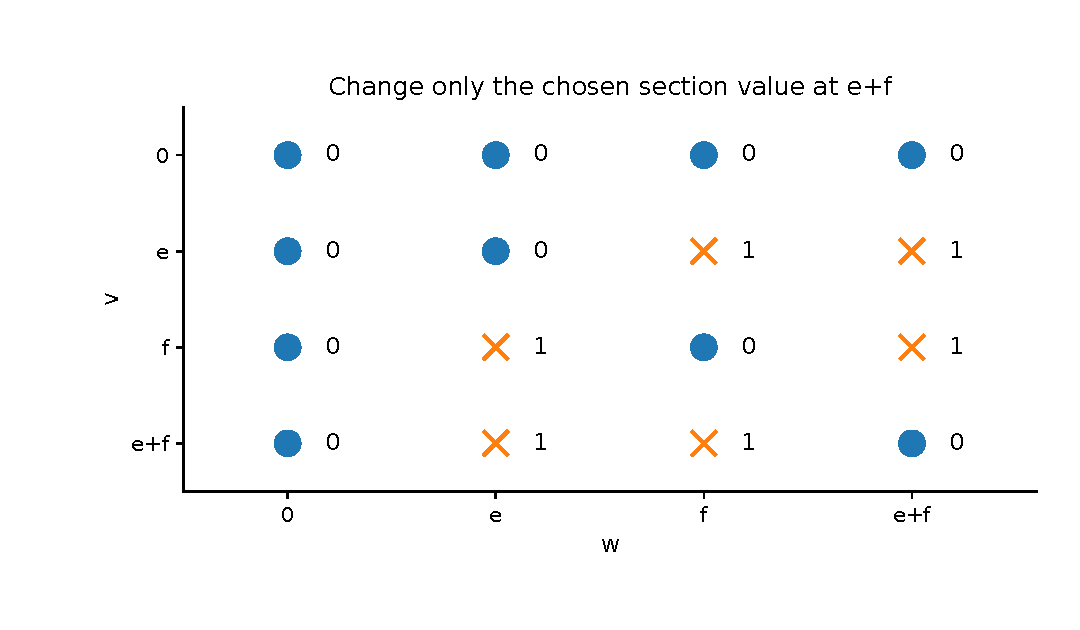
\includegraphics[width=\linewidth]{figures/V21.pdf}\end{center}
Start from the ordered section $\sigma(x,y)=X^xZ^y$ in the dihedral example. Change only $\sigma(e+f)$ by a central sign. Write the sign function as $a(v)=\mathbf1_{v=e+f}$. The displayed entries are the resulting cocycle differences
\[
\Delta c(v,w)=a(v)+a(w)+a(v+w)\in\F_2.
\]
Every diagonal entry is zero, so every square is unchanged. But $\Delta c(e,f)=1$. A map fixing the specified generating lifts cannot also implement the changed assignment at $e+f$. The cross marks a nonzero product discrepancy, not failure of the two extensions to be isomorphic in some other way.

This is why the native certificate needs all specified section products, not only a quadratic table. When the entire section is transported through one homomorphism, those products are retained automatically. When the target section is independently prescribed, its pointwise assignments must be checked. The distinction concerns what is fixed, not a contradiction in extension theory.
\vfill\PlateSource{Exact cocycle counterexample}{Part III, Section 26.3}{68}
